\documentclass{ITaSconf}


\usepackage[russian]{babel}
\usepackage{url}

\usepackage[T2A]{fontenc}
\usepackage[utf8]{inputenc}

\usepackage{graphicx}
\graphicspath{{pic/}}
\DeclareGraphicsExtensions{.pdf,.png,.jpg,gif}
\usepackage{caption}
\usepackage{indentfirst}
\usepackage{misccorr}
\usepackage{amsmath}
\usepackage{indentfirst}
\setlength\parindent{4ex}
\usepackage{fancyhdr}
\usepackage{fixmath}






\begin{document}
\title{Сравнение различных методов декодирования $q-$ных кодов по максимуму апостериорных вероятностей}

\author{
Браславский И.А.\\
 \begin{affiliation}
    ИППИ РАН
  \end{affiliation}\\
  \email{braslavskii@phystech.edu}
\and
Фролов А.А.\\
 \begin{affiliation}
    ИППИ РАН
  \end{affiliation}\\
  \email{alexey.frolov@iitp.ru}
}


\maketitle

\begin{abstract}
  
В работе рассмотрены  и описаны различные методы декодирования кодов с проверкой на четность над полем $GF(q)$. Представлены результаты моделирования  алгоритмов при передаче кодового слова по каналу с аддитивным белым гауссовским шумом. 
\end{abstract} 

\section{Введение}
Мотивацией к написанию было упрощение декодирования недвоичных МПП-кодов.
Декодирование кодов с проверкой на четность над полем $GF(q)$ является наиболее сложной частью декодера МПП-кодов, поэтому данная работа посвящена сравнению различных алгоритмов декодирования таких кодов.
\label{sec:introduct}

\section{Описание кодовой конструкции}
\label{sec:opisanie}

Рассмотрим случай, когда сообщение состоит из $k$ информационных символов и $1$ проверочного. Пусть для информационного вектора $\mathbold{u}=(C_1,C_2...C_k)$, где $ C_i \in GF(q) $, проверочный символ строится как линейная комбинация $C_i$: 
$$C_n=\sum_{i=1}^k \alpha_i C_i$$
где $\alpha_i \in GF(q)$.

Пусть $q=2^r$, тогда спользуя свойство конечных полей характеристики 2: 
$$\beta \in GF(2^n)\Rightarrow\beta+\beta=0,$$ 
получим тождество: 
$$\sum_{i=1}^n \alpha_i C_i=0$$ 
Для того, чтобы из вектора $\mathbold{u}$ получить кодовый вектор, можно домножить его на порождающую матрицу $G$, где 

\begin{equation}\label{eq:pormatrix}
G = \left( \begin{array}{ccccccc}
1 & \dots  & 0 & \alpha_i \\
\vdots       &\ddots &  \vdots &  \vdots \\ 
0 & \dots  &  1&\alpha_n \end{array} \right)  
  \end{equation}

Найдем $\mathbold{v}$:
\begin{equation}\label{eq:kod}
\mathbold{u}G=\mathbold{v}=(C_1 , C_2 \dots C_k,\sum_{i=1}^k \alpha_i C_i)
 \end{equation}
Проверочная матрица $H$ будет иметь вид:
\begin{equation}H = \left( \begin{array}{ccccccc}\label{eq:H}
\alpha_1 & \alpha_2 &  \dots & \alpha_k & \alpha_n \end{array} \right) \end{equation}

Рассмотрим ситуацию наличия помех, создающих одиночную ошибку. Тогда принимающая сторона вместо кодового вектора $\mathbold{v}$  получит искаженный вектор $\mathbold{h}$. Вектор  можно представить в виде суммы
$\mathbold{v}+\mathbold{e}$ , где $\mathbold{e}$  - это вектор ошибки. Домножим $\mathbold{h}$ на $H^T$:
\begin{equation}\label{eq:syndrom}
 \mathbold{h}H^T=(\mathbold{v}+\mathbold{e})H^T=\mathbold{e}H^T
 \end{equation}
 
 Данный код способен обнаружить $1$ одиночную ошибку, но не исправить ее, так как, хоть нам и известно значение ошибки, мы не можем определить номер искаженного символа.

\section{Описание канала}
\label{sec:chanel}

Для передачи данных нам удобно будет пользоваться 8-ичной фазовой манипуляцией ($8psk$).

\begin{figure} [h]
\center{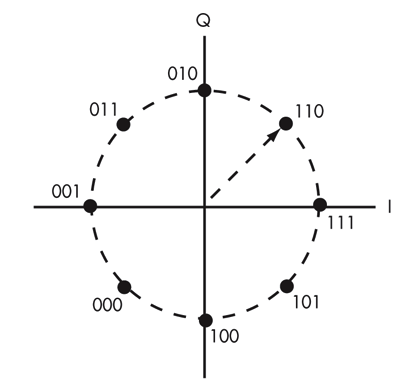
\includegraphics[scale=0.55]{psk.png}}
\caption{фазовая диаграмма $8psk$}
\label{fig:image}
\end{figure}

 Рассмотрим случай канала с аддитивным белым гауссовским шумом ($AWGN$), тогда каждому передаваемому символу $x_i$ можно поставить в соответствие $\mathbold{s_i}$ - точку на фазовой диаграмме, а каждому полученному символу $y_0$ - точку ($\mathbold{s_0}+\mathbold{n})$, которая в процессе передачи переходит в точку $(\mathbold{s_i}+\mathbold{n})$ 
Где аддитивный шум $\mathbold{n}$ подчиняется Гауссовской функции распределения вероятности c плотностью:
\begin{equation}\label{eq:gaus}
p(x)=\frac{1}{\sqrt{2\pi\sigma^2}}\exp{\frac{-(-x-\mu)^2}{2\sigma^2}}, где \mu=0, \sigma^2=\frac{N_0}{2}
 \end{equation}
где $N_0$ - спектральная плотность шума.

Тогда условная вероятность полученного символа $y_i$ при данном переданном $x_0$:

\begin{equation}\label{eq:probab}
p(y_i|x_i)=\frac{1}{\sqrt{\pi N_0}}\exp{\frac{-r_i^2}{N_0}}
 \end{equation}
 где $\mathbold{r_i}=(\mathbold{s_0}+\mathbold{n}-\mathbold{s_i})$ 
 	
Пронормируем вероятности: 
\begin{equation}\label{eq:normprobab}
Pr(y_i|x_i)=\frac{\frac{1}{\sqrt{\pi N_0}}\exp{\frac{-r_i^2}{N_0}}}{\sum_{j=1}^8\frac{1}{\sqrt{\pi N_0}}\exp{\frac{-r_j^2}{N_0}}}
=\frac{\exp{\frac{-r_i^2}{N_0}}}{{\sum_{j=1}^8\exp{\frac{-r_j^2}{N_0}}}}
 \end{equation}
 
 Проделав эту операцию для каждого из 7 полученных символов кодового слова, мы получим матрицу условных вероятностей: 
 
 \begin{equation}\label{eq:probmatrix}
W = \left( \begin{array}{ccccccc}
Pr(y_1|x_1) & \dots  &  Pr(y_7|x_1) \\
\vdots        &\ddots &  \vdots \\ 
Pr(y_1|x_8) & \dots  &  Pr(y_7|x_8) \end{array} \right)  
  \end{equation}
\section{Алгоритм построения решетки}
\label{sec:trellis}

Решетка - это ориентированный граф с периодической
 повторяющейся структурой узлов (ячеек). Узлы собраны в группы, проиндексированные параметром глубины $k$. 
Ребра проведены между двумя определенными парами узлов на глубине $k$  и на глубине $k+1.$ Направления ребер следуют от узлов на $k$ глубине  к узлам $k+1.$ Каждый узел на глубине  $k$ определен  вектором длины $n-k$ над полем $GF(q).$ Назовем его  $s_i(k)$  Решетка является методом компактной записи всех $q^k$ кодовых слов. Каждое отдельное кодовое слово соответствует своему пути в решетке. 

Опишем алгоритм построения путей: 
\begin{enumerate}
 \item На глубине  $k=0$ решетка будет содержать только один узел - нулевой кортеж. Назовем его $S_0(0).$
 \item Для каждого $k=0,1...(n-1)$  узел строится рекурсивно по формуле:
\begin{equation}\label{eq:rec} 
 S_j(k+1)=S_i(k)+\beta_j\bullet h_{k+1}
 \end{equation}
 где $j=0,1...(q-1),$ $\beta_j\in GF(q)$
 \item Удаляются все узлы, не приводящие к нулевому состоянию на глубине $n.$
\end{enumerate}
 
	Для $k=0$ существует только одно состояние узла решетки: $S_0(0).$ Для $k=1$ существует $q$ состояний, а именно: $\beta_j(\mathbold{h_1}),$ $j=0,1...(q-1)$. Для произвольной глубины $1\le k\le n$ у нас будут состояния $\beta_{j1}(\mathbold{h_1})+\beta_{j2}(\mathbold{h_2})+...+\beta_{jk}(\mathbold{h_k}).$ Где '$+$' - это оператор сложения для векторов с компонентами из $GF(q).$ 
	
	Число состояний на любой глубине не может превышать $q^{n-k},$ числа различных $(n-k)$ кортежей с элементами из $GF(q)$
	
	Рассмотрим линейный код ~\eqref{eq:kod} c $n=7$ и $q=8$. Подставляя элементы в рекурсивную формулу 
~\eqref{eq:rec}, а затем удаляя  все ненулевые элементы на глубине $n$, мы получим решетку, в которой каждый узел на глубине $k$ соединен с каждым узлом на глубине $k+1$
	  
\begin{figure} [h]
\center{\includegraphics[scale=0.5]{trellis.png}}
\caption{решетка для кода~\eqref{eq:kod} c $n=7$ и $q=8$}
\label{fig:image}
\end{figure}
Отметим, что для декодирования нет необходимости вычеркивать нежелательные места узлов в решетке.

\section{Алгоритм Витерби}
\label{sec:viterbi}

Пусть на вход декодера нам поступает матрица (\ref{eq:probmatrix}), тогда функция максимального правдоподобия для кодового слова $\mathbold{x}$ будет иметь вид:
\begin{equation}\label{eq:LLR}
Pr(\mathbold{y}|\mathbold{x})=\prod_{i=1}^n\frac{\exp{\frac{-r_i^2}{N_0}}}{{\sum_{j=1}^8\exp{\frac{-r_j^2}{N_0}}}}=\prod_{i=1}^n z_i(y_i,x_i)= Z(\mathbold{x})
 \end{equation}
Декодер максимального правдоподобия позволяет найти наибольшее значение $Z(\mathbold{x})$

Декодер Витерби - это рекурсивный алгоритм, при котором многие кодовые слова могут быть исключены из рассмотрения в процессе максимизации $Z(\mathbold{x})$.
Каждому узлу $S_i(k)$ на глубине $k$ поставим в соответствие действительное число   $V(S_i(k))$, используя следующее правило:
\begin{enumerate}
 \item Для $k=0$ зададим $V(S_0(0))=0$

\item Для каждого узла $S_l(k+1)$ на глубине $k+1 $ вид  $V(S_l(k+1))$ от $V(S_i(k))$ зададим следующим образом:
\begin{equation}\label{eq:LR}
V(S_l(k+1)) = \boldsymbol{\max_{\beta_j \in GF(q)}} [V(S_i(k))\times L(x_{k+1}|\beta_j)]
 \end{equation}
 где $k=0,1..(n-1)$, $i=1..q$, $S_l(k+1)=S_i(k)+\beta_j\times\ h_{k+1}$
 
 \item Оставляем только один путь к $V(S_l(k+1))$ от того $S_i(k)$, который дает максимум в формуле выше
 \item На шаге $k=n$ последовательность  из $\beta_j$ единственного пути от нулевого кортежа на глубине $k=0$ к нулевому кортежу на глубине $k=n$ даст кодовое слово $\mathbold{x}$, которое максимизирует $Z(\mathbold{x})$
\end{enumerate}  

Таким образом, алгоритму требуется $O(n\times\left|{q}\right|^2)$ времени.

\section{BCJR}
\label{sec:vBCJR}

Рассмотрим $q$-ный блоковый, линейный код ($\ref{eq:kod}$) и последовательность $\mathbold{y}=[y_1,y_2...,y_n]$ на выходе канала ($\ref{eq:probmatrix}$). Запишем апостериорные вероятности ($APP$) символов $x_i \in ({0,1,...,q-1})$ используя формулу полной вероятности:
$$p(x_i=x|\mathbold{y})=\frac{p(x_i=x,\mathbold{y})}{p(\mathbold{y})}$$
Где $p(x_i=x,\mathbold{y})$ есть сумма вероятностей всех кодовых слов, где $i$-ый символ равен $x$. 
Сложность вычислений по формуле пропорциональна числу кодовых слов в коде. 

Чтобы упростить вычисления воспользуемся решетчатым представлением кода, для суммирование по кодовым словам мы заменим суммированием по состояниям в узлах решетки $\eqref{eq:rec}$. Обозначим состояние источника на глубине $j$ за $S_j$.
Для удобства обозначим подпоследовательности $y$, как $y_i^j=(y_i,y_{i+1}\dots y_j)$.
Целью декодера является исследование последовательности $\mathbold{y}=y_1^n$ и оценка $APP$ состояний и переходов цепи т.е условных вероятностей:
$$Pr(s_{j-1}=m|\mathbold{y})=\frac{Pr(s_j=m,\mathbold{y})}{p(\mathbold{y})}$$
$$Pr(s_{j-1}=m',s_j=m|\mathbold{y})=\frac{Pr(s_{t-1}=m',s_j=m,\mathbold{y})}{p(\mathbold{y})}$$
Решетчатая диаграмма показывает нам прогрессию во времени последовательность состояний $S_j$. Для каждого состояния решетки $S_j$ существует единственный путь на решетке.
Обозначим $APP$ перехода как
$$\sigma_j(m',m)=Pr(s_{j-1}=m',s_j=m,\mathbold{y}),$$
а $APP$ состояния как 
$$\lambda_j(m)=Pr(s_{j-1}=m,\mathbold{y}).$$
Для принятого вектора $\mathbold{y}$ $Pr(\mathbold{y})$ является константой, которую можно получить из декодера, поэтому для получения искомых $APP$ мы можем нормализировать $\sigma_j(m',m)$ и $\lambda_j(m)$.
Условно разобьем событие $(s_{j-1}=m',s_j=m,\mathbold{y})$ на 'прошлое', 'настоящее' и 'будущее'.
$$\sigma_j(m',m)=Pr([s_{j-1}=m',y_1^{j-1}],[s_j=m,y_j],[y_{j+1}^n])$$
По формуле совместной вероятности можно получить: 
$$Pr(A,B,C)=Pr(A)Pr(B|A)Pr(C|AB)$$
Введем вспомогательные функции вероятности
$$\alpha_j(m)=Pr(A)=Pr(s_j=m,{y_1}^j)$$
$$\gamma_j(m',m)=Pr(B|A)=Pr(s_j=m,y_j|s_{j-1}=m',y_1^{j-1})=$$$$=Pr(s_j=m,y_j|s_{j-1}=m')$$
$$\beta_j(m)=Pr(C|AB)=Pr(y^{n}_{j+1}|s_{j-1}=m',s_j=m,y^{j}_1=Pr(y_{t+1}^n|s_j=m)$$
Тогда можно записать, что 
$$\sigma_j(m',m)=\alpha_{j-1}(m')\gamma_j(m',m)\beta_j(m)$$
$$\lambda_j(m)=\alpha_j(m)\beta_j(m)$$
Теперь наша задача - это получение рекурретных соотношений для $\alpha_j,\beta_j$ и $\gamma_j$ 
Запишем формулу полной вероятности для $\alpha_j(m)$ как
$$\alpha_j(m)=\sum\limits_{m'=0}^{M-1}Pr(s_{j-1}= m',s_j=m,y_1^j)=$$$$=\sum\limits_{m'}Pr(s_{j-1}=m',y_1^{j-1})Pr(s_j=m,y_j|s_{j-1}=m')=$$$$=\sum\limits_{m'}\alpha_{j-1}(m')\gamma_j(m,m')$$
Cреднее равенство вытекает из того факта, что события после глубины $j-1$ не зависят от $y_1^{j-1}$, если $s_{j-1}$ известно. Для $j=0$ мы имеем граничные условия $ \alpha_0(0)=1$ и $\alpha_0(m)=0,$ при $m\neq0$.

	Аналогично, но двигаясь с другой стороны решетки получим соотношение для $\beta_j$
$$\beta_j(m)=\sum\limits_{m'=0}^{M-1}Pr(s_{j+1}=m',y_{j+1}^n|s_j=m)=$$$$=\sum\limits_{m'}Pr(s_{j-1}=m',y_{j+1},y_{j+2}^n|s_t=m)=$$$$=\sum\limits_{m'}Pr(s_{j+1}=m',y_{j+1}|s_t=m)Pr(y_{j+2}^n|s_{j+1}=m')=$$$$=\sum\limits_{m'}\beta_{j+1}(m')\gamma_{j+1}(m',m)$$
Граничные условия: $ \beta_n(0)=1$ и $\beta_n(m)=0,$ при $m\neq0$.

Для применения формул для $\alpha_j(m)$ и $\beta_j(m)$ нужно знать значения $\gamma_j(m',m)$:
$$\gamma_j(m',m)=Pr(s_j=m,y_j|s_{j-1}=m')=p(x_j)p(y_j|x_j)$$ 
Пусть С - множество всех пар $(m',m)$, которым соответствует значение $x_j$, тогда 
$$p(x_j|\mathbold{y}) = \frac{\sum_{(m',m)\in C}\sigma_j(m',m)}{p(\mathbold{y})}$$ 
Пользуясь полученным распределением апостериорных вероятностей можно легко найти наиболее вероятное кодовое слово $\mathbold{x}=[x_1, x_2 \dots x_k, x_n]$

\section{Моделирование}
\label{sec:model}

Моделирование производилось методами имитационного моделирования с использованием среды MatLab для кода (\ref{eq:kod}) длины $n = 7$ над полем $GF(8)$. В качестве канала был выбран канал с аддитивным белым гауссовским шумом (AWGN) и двосьмеричной фазовой манипуляцией (8PSK). 

\begin{figure} [h]
\center{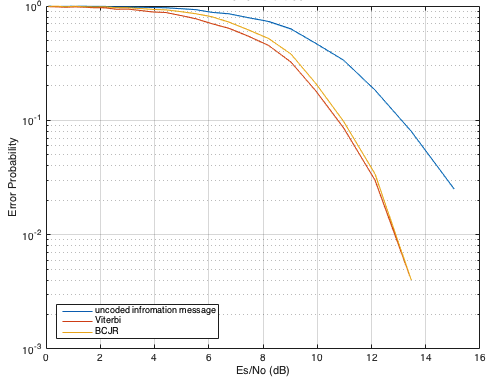
\includegraphics[scale=0.53]{oshibkanablock1.png}}
\caption{Зависимость вероятности ошибки на блок от отношения сигнал-шум на кодовый символ}
\label{fig:block}
\end{figure}

\begin{figure} [h]
\center{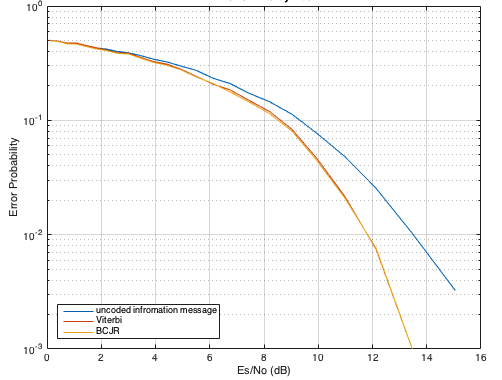
\includegraphics[scale=0.53]{oshibkanasymbol1.png}}
\caption{Зависимость вероятности ошибки на символ от отношения сигнал-шум на кодовый символ}


\label{fig:block}
\end{figure}

Результаты моделирования показывают, что вероятности ошибки на символ у алгоритма  BCJR незначительно меньше, чем у  алгоритма Витерби.

В свою же очередь вероятность ошибки на символ у алгоритма Витерби заметно ниже, чем у алгоритма BCJR.

Для контраста также предоставлен график вероятности ошибки для демодуляции незакодированного сообщения. 


\begin{figure}
\begin{thebibliography}{9}

\bibitem{wolf}
JACK K. WOLF, Efficient Maximum Likelihood Decoding of Linear Block Codes Using a Trellis,
IEEE TRANSACTIONS ON INFORMATION THEORY, VOL. IT-24, NO. 1, JANUARY 1978

\bibitem{BCJR}L. R. BAHL, J. COCKE, F. JELINEK, AND J. RAVIV, Optimal Decoding of Linear Codes for Minimizing Symbol Error Rate, IEEE TRANSACTTONS ON INFORMATION THEORY, MARCH 1974
\bibitem{kudr}Б. Д. Кудряшов, Основы Теории Кодирования
\end{thebibliography}
\end{figure}

\end{document}
